\documentclass[11pt,letterpaper,twocolumn,english,DIV=calc]{scrartcl}
\usepackage{fontspec}
\usepackage[footsepline]{scrlayer-scrpage}
\setmainfont[Ligatures=TeX]{TeX Gyre Heros}
\setsansfont[Ligatures=TeX]{Linux Biolinum O}
\setcounter{secnumdepth}{2}
\setcounter{tocdepth}{2}
\usepackage{color}
\usepackage{array}
\usepackage{float}
\usepackage{units}
\usepackage{url}
\usepackage{enumitem}
\usepackage{graphicx}
\usepackage{setspace}
\usepackage[authoryear]{natbib}
\usepackage[unicode=true, bookmarks=true, bookmarksnumbered=false,
			bookmarksopen=false, breaklinks=false, pdfborder={0 0 0},pdfborderstyle={}, backref=false, colorlinks=true]{hyperref}
\hypersetup{pdftitle={Polish Horseshoes, Brookline Rules},
			pdfauthor={Phillip Anderson}, pdfsubject={polish horseshoes},
			pdfkeywords={beer, frisbee, polish, horseshoes, brookline}}

\makeatletter

%%%%%%%%%%%%%%%%%%%%%%%%%%%%%%%%%%%%%%%%%
% This template is based on:
%
% Large Colored Title Article LaTeX Template, Version 1.1 (25/11/12)
% Downloaded from: http://www.LaTeXTemplates.com
% Original author: Frits Wenneker (http://www.howtotex.com)
% License: CC BY-NC-SA 3.0 (http://creativecommons.org/licenses/by-nc-sa/3.0/)
%%%%%%%%%%%%%%%%%%%%%%%%%%%%%%%%%%%%%%%%%

\newcommand{\rev}{Revision 6}
\newcommand{\currentyear}{2019}

\newcommand{\proposed}{{\color{DarkRed} \textsc{(Proposed) }}}
\usepackage{draftwatermark}

%\usepackage[protrusion=true,expansion=true]{microtype} % Better typography
\usepackage[svgnames]{xcolor}
\usepackage[format=plain, labelfont=bf,up, textfont=up]{caption} % Custom captions under/above floats in tables or figures
\usepackage{booktabs} % Horizontal rules in tables
\usepackage{fix-cm}	 % Custom font sizes - for the initial letter in the doc
\usepackage{sectsty} % Enables custom section titles
\usepackage{lastpage}
\usepackage{fontspec}
\usepackage{fontawesome}

\usepackage{lettrine} % Package to accentuate the first letter of the text
\newcommand{\initial}[1]{ % Defines the command and style for the first letter
	\lettrine[lines=2, lhang=0.35, nindent=0.1em, loversize=0.25]{
		\color{DarkRed}{\textsf{#1}}}{}}

\hypersetup{urlcolor=DarkRed, linkcolor=DarkRed}

\usepackage{tikz}
\usetikzlibrary{arrows,patterns}
%\setlength{\intextsep}{0cm plus1cm minus1cm}

\ifoot{\footnotesize\rev}
\cfoot{\footnotesize\copyright\ 2012-\currentyear\ 
	   by Phillip Anderson. CC BY-NC-ND}

\ofoot{\footnotesize Page \thepage\ of \pageref{LastPage}} % "Page 1 of 2"

\deffootnote[0.7em]{0pt}{1.6em}{\makebox[0.7em][l]{\textsuperscript\thefootnotemark}}

\usepackage{titling} % Allows custom title configuration

\newcommand{\HorRule}{\color{Black} \rule{\linewidth}{1pt}} % Defines the gold horizontal rule around the title

\pretitle{\vspace{-85pt} \begin{flushleft} \HorRule \fontsize{50}{50}  \color{DarkRed} \selectfont} % Horizontal rule before the title

\title{\textsf{Polish Horseshoes}} % Your article title

\posttitle{\par\end{flushleft}\vskip .0em} % Whitespace under the title

\preauthor{\color{DarkRed} \huge\hspace{2pt}\textsf{Brookline Rules} %\begin{flushleft}\large \lineskip 0.5em \usefont{OT1}{phv}{b}{sl} \color{DarkRed}
} % Author font configuration

\author{}

\postauthor{\footnotesize \color{Black} % Configuration for the institution name
%University of  % Your institution

%\par\end{flushleft}
\HorRule

\hfill \color{Black}\large \rev: \today \vspace{-25pt}} % Horizontal rule after the title

\setlength{\columnsep}{4ex}
\date{} % Add a date here if you would like one to appear underneath the title block
\setlist[enumerate, 1]{label=\thesection.\arabic*, parsep=0pt}
\setlist[enumerate, 2]{leftmargin=1.4em}

\makeatother

\usepackage{polyglossia}
\setdefaultlanguage[variant=american]{english}
\begin{document}
\maketitle

\thispagestyle{headings}

\initial{P}olish Horseshoes is a yard game where opponents make alternating attempts to hit and defend an empty beer bottle perched on a pole to score points, all while holding a beverage in one hand.
The game seems to have originated in the early 2000's, and is now known by a variety of alternate names such as Beersbee, Frisbeener, and Spanish Horseshoes, among others.%
\footnote{\url{http://en.wikipedia.org/wiki/Polish_horseshoes}}
Many variations exist for the rules and, although they are broadly similar on the main points, most descriptions found online are quite vague or over-simplified. 
A game this good needs and deserves a solid, common set of rules.

We first came across Polish Horseshoes late in 2010 via a friend and were immediately hooked. 
\emph{Brookline Rules} is our variation of Polish Horseshoes, developed and fine-tuned over the years in and around Boston, Massachusetts. 
It is now a staple of picnics, cookouts, and other outdoor events whenever the weather is agreeable and occasionally even when it is not. 
Described here are our official rules, recommendations for equipment, and suggestions for playing safely. 
We hope you enjoy the game as much as we have.

\begin{figure}[H]
	\centering{}
	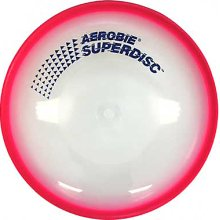
\includegraphics[width=0.24\textwidth]{images/superdisc}{\footnotesize{}Source:
	\href{http://www.aerobie.com}{aerobie.com}}
\end{figure}


\part*{Equipment}

Only a few bits are needed to play, most of which are easy to find.
This is what you will need:

\begin{description}[font=\large, leftmargin=0.5em]
	\item [{Aerobie® Superdisc™:}] 
		The weight, controllability, and soft edge of these discs make them ideal for play.\footnote{\url{http://www.aerobie.com/products/superdisc.htm}} 
		Lighter discs tend to be cheap and difficult to control, and heavier discs or those with hard edges are prone to destroying bottles very quickly. 
	\item [{Empty bottles (2):}] 
		Use standard $355\,\mbox{mL}$ bottles and keep spares on hand in case of breaks during play.
		Fill with expanding polyurethane foam to greatly reduce the likelihood of shattering for a negligible increase in weight. 
	\item [{Plastic cups (2):}] 
		$16\,\mbox{oz.}$ cups work well and are easy to find. 
		These wear out frequently so keep extras on hand or patch with packaging tape.
	\item [{Poles (2):}] 
		These are the most difficult to source and may require some creativity. 
		Standard poles are $19\,\mbox{mm}$ diameter and $1.2\,\mbox{m}$ long with a pointy end for the ground and a cap on which to balance the bottle. 
		Ski poles are traditional, but poles can otherwise be fashioned from fiberglass rods. 

		Tennis balls make good caps for a ball-and-socket joint if the plastic cups fit. 
		The pointy end may require manufacturing a spike which can be secured by cutting a small slot on the end and tightening with a hose clamp.
	\item [{Tasty~beverages:}] 
		All players will need a tasty beverage of their choice, or equivalent, to occupy one hand during play. 
		Glass vessels are at risk of shattering if hit, so aluminum cans are recommended. 
\end{description}

\begin{figure*}[!ht]
	\begin{centering}
		%\usetikzlibrary{arrows,patterns}
\begin{tikzpicture}[line cap=round,line join=round,>=stealth,x=1.1cm,y=1.1cm]

% court specifications
\def\w{2.5} % width of court
\def\pp{10} % minimum pole to pole distance
\def\d{2.5} % depth of player area
\def\pzi{0.4} % depth that pole zone is inset into player area
\def\pzw{1.6} % width of pole zone
\def\pzd{0.5} % depth of pole zone
\def\extra{0.5} % how much to extend guide lines
\def\bt{0.1} % border thickness for player area

% convenience definitions
\def\hw{\w/2} % half the width of the court
\def\hpp{\pp/2} % half the minimum pole to pole distance

% entire court area
\draw[fill=green!25] (-\hpp+\pzi-\d,-\hw) rectangle (\hpp-\pzi+\d,\hw);

\foreach \i in {-1,1}{
  % player zones
  \draw[fill=brown] ({\i*(\hpp-\pzi)}, -\hw) rectangle ++(\i*\d, \w);
  \draw[fill=brown!20] ({\i*(\hpp-\pzi+\bt)}, -\hw+\bt) rectangle ++({\i*(\d-2*\bt)}, \w-2*\bt);
}

% pattern for middle zone
\fill[pattern=crosshatch dots, pattern color=black!40] 
	(-\hpp-\pzd/2,-\hw) rectangle (\hpp+\pzd/2,\hw);

% half court line and label
\draw[dashed] (0,-\hw) -- (0,\hw+\extra/2) node[above] {half court};

\foreach \i in {-1,1}{
  % pole zones
  \draw[rounded corners=5*\pzd, fill=yellow!30] (\i*\pp/2,-\pzw/2) rectangle ++(\i*\pzd,\pzw);
    
  % bottles
  \draw[color=red, fill=red] ({\i*(\hpp+\pzd/2) +\i*0.08}, rand/3) circle(.1) coordinate(cup);
  \draw[thin, color=black,fill=brown] (cup) circle (0.08) circle(0.03);

  % bottle plane lines and labels
  \draw[dashed] ({\i*(\hpp+\pzd/2)},0) +(0,-\hw) -- +(0,\hw+\extra/2) node[above] {$bp$};
  \draw[dashed] (\i*\hpp, -\hw-\extra/2) -- ++(0, \hw);
}
\draw[dashed] (\hpp+\pzd, -\hw-\extra/2) -- ++(0, \hw);

% distance callouts for middle zone, court width, pole zone depth, and player area depth, respectively
\draw[thick,|<->|] (-\hpp, -\hw-\extra) -- node[fill=white] {\pp\ m} +(\pp,0);
\draw[thick,|<->|] (\hpp-\pzi+\d+\extra,-\hw) -- node[fill=white, xshift=7] {\w\ m} +(0,\w);
\draw[thick,|<-] (\hpp+\pzd,-\hw-\extra) -- node[fill=white, anchor=west, xshift=0] {\pzd\ m} +(\pzd,0);

% \draw[thick,|<->|] (\pp/2,-\w/2-2*\extra) -- node[fill=white, anchor=north, yshift=-5] {\pzd\ m} +(\pzd,0);
% \draw[thick,|<->|] (\pp/2+\pzd,-\w/2-\extra) -- node[fill=white] {\sim\d\ m} +(\d,0);
% \draw (0,0) circle(1);

%players left (top, bottom) and right (top, bottom)
\begin{scope}[thick, x=2mm, y=2mm, xshift=-7cm, xscale=1, rotate=-20]
	\draw[line width=1.8mm] (0, 1.65) -- ++(0.8, .4) -- ++(1.2, 0.1) coordinate(hand1);
	\draw[color=black!20!red,line width=1.3mm] (0, 1.65) -- ++(0.8, .4) -- ++(1.2, 0.1);
	\draw[line width=1.8mm] (0, -1.65) -- ++(.5, -.5) -- ++(.7, -.3) coordinate(beer1);
	\draw[color=black!20!red, line width=1.3mm] (0, -1.65) -- ++(.5, -.5) -- ++(.7, -.3);
	\draw[thin, fill=brown!60] (hand1) ellipse(0.5 and 0.4) (beer1) ellipse(0.6 and 0.4);
	\draw[thin, fill=brown] (beer1) +(0,0.3) circle(0.45) circle(0.18);
	\draw[fill=red] ellipse(.8 and 2);
	\draw[fill=brown!50!black] (.1,0) circle(1);
\end{scope}
\begin{scope}[thick, x=2mm, y=2mm, xshift=7cm, xscale=-1, rotate=-20]
	\draw[line width=1.8mm] (0, 1.65) -- ++(0.8, .4) -- ++(1.2, 0.1) coordinate(hand1);
	\draw[color=blue!60,line width=1.3mm] (0, 1.65) -- ++(0.8, .4) -- ++(1.2, 0.1);
	\draw[line width=1.8mm] (0, -1.65) -- ++(.5, -.5) -- ++(.7, -.3) coordinate(beer1);
	\draw[color=blue!60, line width=1.3mm] (0, -1.65) -- ++(.5, -.5) -- ++(.7, -.3);
	\draw[thin, fill=brown!60] (hand1) ellipse(0.5 and 0.4) (beer1) ellipse(0.6 and 0.4);
	\draw[thin, fill=brown] (beer1) +(0,0.3) circle(0.45) circle(0.18);
	\draw[fill=blue!70] ellipse(.8 and 2);
	\draw[fill=brown!50!black] (.1,0) circle(1);
\end{scope}

\end{tikzpicture}
\vspace{-5mm}\par
	\end{centering}
	\caption{
		Top-down schematic of the court. 
		Poles (brown dots) can be placed anywhere within the pole zones (yellow regions). 
		Players stand behind the \emph{bottle plane} ($bp$) on their respective side.\label{fig:court}
	}
\end{figure*}


\part*{Court}%

A polish horseshoes court is composed of a $10\,\mbox{m\,\times\,} 2.5\,\mbox{m}$ clearing bookended by $0.5\,\mbox{m}$ wide pole zones and player boxes, as shown in figure~\ref{fig:court}.
Edges of the court do not prescribe bounds, but they may be marked by physical boundaries such as fences or walls.
In fact, there are no bounds per~se, but regions deemed particularly undesirable for the disc (windows, bodies of water, rough terrain, neighbors' yards, etc.) are designated as \emph{traps}.

The court should be free of traps, but low obstructions and uneven terrain are allowed in the central area.
Player boxes must be clear, reasonably flat, and at a similar elevation.
\emph{Breakers} such as rocks or other hard objects may be located along the perimeter.
Pole zones should contain a packable dirt or clay mixture so that the poles are easily planted and supported.

Players face each other from their respective boxes on opposing ends of the court and set thier poles.
The pole is set by planting it anywhere in the pole zone, placing an inverted plastic cup over the cap to form a flat base, and balancing an empty bottle on top, as shown in figure~\ref{fig:pole-setup}. 
The cup is considered to be part of the pole.
 
Players position themselves behind their own \emph{bottle plane}, an imaginary plane extending vertically from the ground through the bottle centerpoint and perpendicular to the long axis of the court.

\begin{figure}[!hb]
	\begin{centering}
		\begin{tikzpicture}[line cap=round,line join=round,>=stealth,x=1mm,y=1mm]

\def\ch{10} %cup height
\def\cdt{8} %cup top diameter
\def\cdb{6.0} %cup bottom diameter

\def\pl{70} %pole length actually 120
\def\pt{7.5} %pole taper length
\def\pd{1.6} %pole diameter
\def\dd{5} %disc diameter
\def\dt{1.9} %disc thickness
\def\balld{6.0} %tennis ball diameter
\def\extra{4} %how much to extend guide lines

\begin{scope}[xshift=0mm,scale=.55]

\draw[rotate=-10] (0,\pl-2) coordinate (B);

%ground
\draw[fill=brown,color=brown] (-4*\extra,-3*\extra) rectangle (32*\extra,0);
\draw[ultra thick, color=black!30!green] (-4*\extra,0) -- (32*\extra,0);
\draw[->, thick] (29*\extra, 2*\extra) node[left] {half court} -- (31*\extra, 2*\extra);

%cup
\draw (B) ++(0, \dt/2+2.5) coordinate(cup);
\draw[red,fill=red!10, thick] (cup) ++(-\cdt/2,-\ch) -- ++(\cdt/2-\cdb/2,\ch) -- ++(\cdb,0) -- ++(\cdt/2-\cdb/2,-\ch) -- cycle;
\draw[black,fill=white,thin] (cup) ++(-\cdt/2,-\ch-.3) rectangle ++(\cdt,.6);
\draw[black,fill=white,thin] (cup) ++(-\cdt/2,-\ch) circle (.5) ++(\cdt,0) circle (.5);

%pole
\begin{scope}[rotate=-10]
\draw[fill=yellow] (-\pd/2,0) rectangle ++(\pd,\pl); %pole
\draw[fill=black] (-\pd/2,\pl) rectangle ++(\pd,-\pl/10); %handle
\draw[fill=gray] (0,-\pt) -- ++(-\pd/2,\pt) -- ++(\pd,0) -- cycle; %spike
\draw[fill=white] (-2*\pd,-0.5) rectangle (2*\pd,0.5); %guard
\draw[fill=green] (B) circle (\balld/2); %tennis ball
\end{scope}

%bottle
\begin{scope}[scale=.25]
\draw[fill=black!50!brown] 
(cup) ++(0,1)
 .. controls ++(-1,0) and ++(1,0) .. ++(-6.6,0)
.. controls ++(-3.2,0.2) and ++(0,-2.5) .. ++(-5.8, 4.2)
.. controls ++(0,1) and ++(0,-1) .. ++(0,47.2)
.. controls ++(0,2.5) and ++(-0.9,-1.4) .. ++(2.3,5.7)
.. controls ++(1.9,3.1) and ++(-0.3,-1.4)   .. ++(2.6,5.3)
 .. controls ++(0.5,2.1) and ++(-0.9,-16.8)  .. ++(1.9, 25.6) 
 .. controls ++(-0.4,0.4) and ++(-0.2,-1.1)  .. ++(-0.2, 3.3)
 .. controls ++(0.2,0.5) and ++(0.2,-0.2)  .. ++(-0.1,1.3) 
.. controls ++(-0.6,0.9) and ++(-1.1, -0.4)  .. ++(1.2,3.5) 
.. controls ++(1.2,0.4) and ++(-2.2,0)  .. ++(4.7, 0.2)

.. controls ++(2.2,0) and ++(-1.2,0.4) .. ++(4.7, -0.2)
 .. controls ++(1.1, -0.4) and ++(.6,0.9) .. ++(1.2,-3.5) 
 .. controls ++(-0.2,-0.2) and ++(-0.2,0.5) .. ++(-0.1,-1.3) 
 .. controls ++(0.2,-1.1) and ++(0.4,0.4) .. ++(-0.2, -3.3)
 .. controls ++(0.9,-16.8) and ++(-0.5,2.1) .. ++(1.9, -25.6) 
.. controls ++(0.3,-1.4) and ++(-1.9,3.1) .. ++(2.6,-5.3)
.. controls ++(0.9,-1.4) and ++(0,2.5) .. ++(2.3,-5.7) 
.. controls ++(0,-1) and ++(0,1) .. ++(0,-47.2)
.. controls ++(0,-2.5) and ++(3.2,0.2) .. ++(-5.8, -4.2) 
.. controls ++(-1,0) and ++(1,0) .. ++(-6.6,0)
;

% bottle planes
\draw[dashed, red, very thick] (10,0) -- ++(0, 450) node[above] {A};
\draw[dashed, blue, very thick] (35,0) -- ++(0, 450) node[above] {B};
\draw[dashed, orange, very thick] (62,0) -- ++(0, 450) node[above] {C};

% discs
\draw[dotted, red, thick] (10, 45) -- (180, 45);
\draw[red, fill=red] (180, 45) -- ++(8, 12) -- node[above] {A} ++(100, 0) -- ++(8, -12) -- cycle;

\draw[dotted, blue, thick] (35, 180) -- (200, 180);
\draw[blue, fill=blue] (200, 180) -- ++(8, 12) -- node[above] {B} ++(100, 0) -- ++(8, -12) -- cycle;

\draw[dotted, orange, thick] (62, 410) -- (220, 410);
\draw[orange, fill=orange] (220, 410) -- ++(8, 12) -- node[above] {C} ++(100, 0) -- ++(8, -12) -- cycle;
\end{scope}
\end{scope}
\end{tikzpicture}

\vspace{-5mm}\par
	\end{centering}
	\caption{
		Pole setup. 
		Pointy end in the ground. 
		An inverted plastic cup covers the cap, creating a flat base for the bottle. 
		Round caps form a ball-and-socket joint with the cup and allow the bottle to be balanced even when the pole is not vertical.\label{fig:pole-setup}
	}
\end{figure}

\clearpage
\part*{Gameplay}

This section describes the rules for a \emph{singles} game, but adjustments for variations such as doubles play can be found in the \nameref{part:variants} section.
	
\section{Basic play and terminology}
\begin{enumerate}
	\item All players must have a tasty beverage or equivalent in one hand during play.
	\item Both players start with 0 points and 10 HP.
	\item \label{enu:alternate_throws} Players alternate throwing the disc, which is \emph{live} at the point of release and \emph{dead} upon contacting any object afterwards.

	\item The disc is considered \emph{catchable} if it crosses the $bp$ (i) between the defender's knees and hairline, and (ii) within $1\mbox{ m}$ to either side of the Defense's bottle, subject to some exceptions.
	\begin{enumerate}
		\item The disc is not catchable if it is within one diameter of an obstacle when it crosses the bottle plane (safety exception).
		\item The disc is not catchable if it lands within one diameter of the $bp$ (steep throw exception).
		\item If catchability is contested, the benefit of doubt usually goes to the Defender.
	\end{enumerate}

	\item The disc is \emph{short} if it comes to rest without crossing the $bp$. 
		Offense has the option to throw a shorted disc from its resting position. 

	\item Catching, blocking, or deflecting the disc before it breaks the $bp$ is \emph{goaltending}, but only if it is live.
	
	\item The disc \emph{hits} if it makes contact with the opponent's pole or bottle, otherwise it \emph{misses}.
	A hit is \emph{direct} if the disc is not dead before contactin the pole or bottle, and \emph{grazing} if it does not result in the bottle falling.

\end{enumerate}

\section{Scoring}
\begin{enumerate}
	\item \label{enu:dropped_point}Offense is awarded one point for throwing a live catchable disc that misses but is not caught (\emph{dropped}). 
	\item \label{enu:bottle-hit}Offense is awarded one point for a direct bottle hit.
	\item Offense is awarded two points for a hit that results in the Defense's bottle touching the ground.
	\item \label{enu:stalwart}Defense is awarded one point if the defender catches the disc and the bottle before they touch the ground after a live non-grazing hit (\emph{stalwart defense}). 

	\item If a throw is goaltended, Offense is awarded points corresponding to the most likely hit.
	\begin{enumerate}
		\item If the goaltender does not have both feet behind the $bp$, Offense is awarded a minimum of two points.
	\end{enumerate}

	\item Points are not awarded for dropped discs, hitting the bottle, or performing a stalwart defense if they would result in a victory (i.e. rules \ref{enu:dropped_point}, \ref{enu:bottle-hit}, and \ref{enu:stalwart} are suspended). Instead, the opponent loses the equivalent in HP.

	\item All rules and penalties stack.
	\item Points and penalties are applied in the chronological order that they occurred.
\end{enumerate}

\section{Winning the game}
There are three ways to end the game.
\begin{enumerate}
	\item \label{enu:win-conditions}Point victory: Play goes to eleven points, win by two.
		Beyond this, players are either tied (\emph{deuce}) or one leads by a single point (\emph{advantage}).
		\begin{enumerate}
			\item Play does not end upon loss of a point (see sections \ref{subsec:clumsiness-and-carelessness} and \ref{subsec:traps} for scenarios), even if the conditions in rule \ref{enu:win-conditions} are met. 
				The penalized player may become \emph{profoundly disadvantaged} or worse under these circumstances.
		\end{enumerate}
	
	\item Not-so-sudden-death: If a player reaches 0 HP, they lose the game.

	\item Fatality: If a bottle cracks or breaks, the owning team loses immediately.
	\begin{enumerate}
		\item If a bottle has only one crack which does not extend below the shoulder, it may be replaced but not defended for the remainder of the game (\emph{ghost bottle} exception).
		\item A cracked ghost bottle cannot be replaced (\emph{no more continues} exception).
	\end{enumerate}
\end{enumerate}

\section{\label{sec:special-scenarios}Special scenarios}

\subsection{\label{subsec:clumsiness-and-carelessness}Clumsiness and carelessness}
\begin{enumerate}[leftmargin=2.8em, label=\thesubsection.\arabic*]
	\item If a player steps over the $bp$ while throwing, no points are awarded (\emph{line fault}). 
	If this throw results in a broken or damaged bottle, the bottle is replaced.
	\item Any player who's tasty beverage suffers a hit by a live disc loses one point.
	\item Dropping one's tasty beverage results in the loss of a point.
	\item Grabbing an undisturbed bottle results in the loss of a point.
	\item Bumping one's own pole or bottle awards the opposing player two points for a pole bump or three points for a bottle bump, unless the bottle is caught. 
	This does not include bottles dropped when resetting.
	\item If a player throws with an unset bottle, they must reset the bottle before the next throw or else are penalized one point.
	\item No points or penalties are given for acts of god, such as the wind blowing the bottle off of the pole.
\end{enumerate}

\subsection{\label{subsec:traps}Traps and redemption shots}
\begin{enumerate}[leftmargin=2.8em, label=\thesubsection.\arabic*]
	\item Throwing the disc into a trap results in the loss of a point.
	\item The thrower is responsible for retrieving the disc from any traps where retrieval is difficult.
	\item If the trap does not have a direct line to the opponent's pole, the thrower may opt to throw the disc back into the court from the trap (\emph{redemption shot}).

	\begin{enumerate}
		\item If the redemption shot knocks the opponent's bottle to the ground, the lost point is regained.
		\item Redemption shots cannot be defended.
		\item If the disc lands in any trap, the thrower loses another point.
		\item Only one redemption shot is allowed per trapped throw.
	\end{enumerate}
\end{enumerate}

\subsection{On fire}
\begin{enumerate}[leftmargin=2.8em, label=\thesubsection.\arabic*]
	\item \label{enu:fire_count} A player who executes three consecutive direct hits is \emph{on fire}.
	The player is \emph{heating up} after the second hit.
	\item Normal play is paused while a player is on fire. 
	The on fire player throws until failing to make a direct hit, at which point fire is lost and that player's fire count returns to zero.
	\item Fire throws cannot be defended, the bottle may not be caught, and points are awarded as if in normal play.
	\item \label{enu:splooshing_1} Consecutive hit count for a player is \emph{splooshed} (reset to zero) if the opposing team makes a 2+ point play.
	\item Consecutive hit count for a player is reset to zero if that player's tasty beverage suffers a direct hit.
	\item Goaltending does not affect any player's fire count.
	\item Ambiguities in \emph{fire} rules may be settled by an appeal to NBA Jam.
\end{enumerate}

\subsection{Extreme events and beverage debts}
\begin{enumerate}[leftmargin=2.8em, label=\thesubsection.\arabic*]
	\item A \emph{shutout} occurs when the losing team does not have a positive score at the end of a game.

	\begin{enumerate}
		\item All losers of a shutout must drink an agreed upon \emph{nasty beverage}.
		\item An additional drink is owed for each point the \emph{losing team}'s score is below zero.
	\end{enumerate}

	\item \emph{Shooting the moon} occurs when the winning team does not have a positive score at the end of a game (by breaking the opponents bottle).

	\begin{enumerate}
		\item All losers of a moon shot must drink an agreed upon \emph{nasty beverage}.
		\item The loser owes a nasty beverage for each point the \emph{winner's} score is below zero.
	\end{enumerate}

	\item \emph{Mutual shame} occurs if neither team has a positive score at the end of a game.

	\begin{enumerate}
		\item All victims of mutual shame must drink a nasty beverage.
		\item The nasty beverage must be chosen from the default list.
		\item Beverage debts from mutual shame may not be wagered, forgiven, canceled, or transferred.
	\end{enumerate}

	\item A \emph{photo-finish} occurs when both teams are tied at the end of a game.
	\item The nasty beverage should be chosen before the game begins.

	\begin{enumerate}
		\item The choice of nasty beverage may be agreed upon or changed at any time if the players involved agree on the new choice.
		\item If players cannot come to an agreement, the default beverage choices are Bud Light with Lime, Smirnoff Margarita, or PBR with a fresh squeezed lime.
		\item In the case of a player shooting the moon, moon shots may be taken to pay beverage debts.
	\end{enumerate}

	\item Beverage debts do not have to be repaid immediately.
	\item Beverage debts may be wagered, forgiven, canceled, or transferred (by trickery if necessary). 
	Debts from mutual shame are an exception.
	\item Beverage debts may be reduced if paid in bulk, at the discretion of the parties owed.
\end{enumerate}

\section{Series and tournament play}
\begin{enumerate}[label=\thesection.\arabic*]
	\item The winner of a fair toss chooses to have first throw or preferred side.
	\item In a series, team sides and first throw alternate after each game.
	\item A set is composed of an odd number of games, typically three.
	\item A match is composed of an odd number of sets, typically one (equivalent in this case).
	\item Each team must use the same bottle for the duration of a match.

	\begin{enumerate}
		\item A broken bottle is replaced for the next game. 
		Replacements must be used for the rest of the match or until they break.
	\end{enumerate}
	\item \proposed Each player may be alloted a fixed number of bottles for the season
	\item \proposed Handicap system for series play.

\end{enumerate}

\part*{Box Scoring System}

\part*{Variants}
\label{part:variants}

Variants are based on the rules for a singles game. Rules listed here extend the base rules where there is no conflict, and supersede where there is.

\section{Doubles}
Four players face off, with the pairs on either side of the court forming a team. 

\begin{description}
	\item{\S\ref{enu:win-conditions}} Play goes to twenty-one points, win by two.
	\item{\S\ref{enu:alternate_throws}} Teams and teammates alternate throws. 
	\item{\S\ref{enu:dropped_point}} Offense is also awarded one point for throwing a live hit if the disc is uncaught.
	\item{\S\ref{enu:fire_count}} Fire counts are tracked per player and not per team.
\end{description}

\section{Di-Polish}
Each side has two poles and two bottles.

\section{Standard Polish}
Each side has a battle standard to the side of the court.

\section{Glossary}
Each side has a battle standard to the side of the court.

\newpage{}

\part*{Back Matter}

\addsec{Credits}

Many thanks to everybody who helped with game development and codifying the rules (in alphabetical order):\medskip{}

\begin{tabular}{>{\raggedright}p{3.5cm}>{\raggedright}p{2.5cm}}
	Phillip Anderson & Julian S.\tabularnewline
	Mike C. & Jon S.\tabularnewline
	Will E. & Konrad S.\tabularnewline
	Mike F. & Matt T.\tabularnewline
	Jon K. & Kristine W.\tabularnewline
	Andrew O. & Dustin W.\tabularnewline
\end{tabular}

\addsec{Disclaimer}

Nobody involved with writing or distributing this document is responsible for injuries that may be caused by playing this game.

\medskip{}\noindent Polish Horseshoes is not sponsored or endorsed by any of the companies mentioned.

\addsec{License}

\copyright\ 2012-\currentyear\ by Phillip Anderson. 

\noindent This work is licensed under the Creative Commons Attribution
- NonCommercial - NoDerivatives 4.0 International License. 
Visit \href{http://creativecommons.org/licenses/by-nc-nd/4.0/}{creativecommons.org} to view a copy of this license.

\begin{figure}[!h]
	
\includegraphics[width=\columnwidth]{images/by-nc-nd}
\end{figure}

\newpage{}

\ \vfill{}

\noindent Visit, contact or follow at the following links for questions, comments, or other communications:

\begin{description}[listparindent=1.cm, font=\normalfont]
	\item[{\faGlobe}] \href{https://github.com/anderson-pa/polish_horseshoes/releases}{https://github.com/anderson-pa/\\\indent polish\_horseshoes/releases}

	\item[\faEnvelopeO] \href{mailto:brpolish@gmail.com}{brpolish@gmail.com}

	\item[\faTwitter] \href{http://www.twitter.com/br_polish}{@br\_{}polish}

	\item[\faTwitch] \href{http://www.twitch.tv/br_polish}{br\_{}polish}
\end{description}

\end{document}
